%******************************************************************************************************
%******************************* Third Chapter ********************************************************
%******************************************************************************************************

\externaldocument{{../Chapter1/chapter1}}
\externaldocument{{../Chapter2/chapter2}}
\externaldocument{{../Chapter4/chapter4}}
\externaldocument{{../Chapter5/chapter5}}
\externaldocument{{../Chapter6/chapter6}}
\externaldocument{{../Chapter7/chapter7}}
\externaldocument{{../Appendix1/appendix1}}
\externaldocument{{../Appendix2/appendix2}}
\externaldocument{{../Appendix3/appendix3}}
\externaldocument{{../Appendix4/appendix4}}
\externaldocument{{../Appendix5/appendix5}}
\externaldocument{{../Appendix6/appendix6}}
\externaldocument{{../Appendix7/appendix7}}

% **************************** Define Graphics Path **************************
\graphicspath{{Chapter3/Figs/}}

%******************************************************************************************************
%******************************************************************************************************
%******************************************************************************************************
%******************************************************************************************************
\chapter{Task One: Path Planning}
\label{task1}

In this report the practical work has been clearly divided into two distinct tasks, allowing us to simplify, shorten, and better organise both the work and the reporting of it. This chapter of the report will discuss the first of the two practical tasks, covering the design, implementation, and testing of the solution for the path planning problem discussed in Section \ref{intro:objectives}. 

The solutions proposed here are intended to be used in conjunction with the chosen mission planning software prior to flight. From this we can assume that any program or application developed in this section is intended to be run on a personal computer of some description, rather than on the UAV itself. 

%******************************************************************************************************
%******************************************************************************************************
\section{Path Planning - Aims}
\label{task1:aims}

This section of work is aimed at producing a system to enable us to both plan and define paths for the UAV to follow. The paths we need to produce must in fact be sections of larger mission plans, and must be used to enable the UAV to travel between the end of one imaging path and the start of the next. Stock ArduPlane can of course offer this, but what it cannot offer is the abilty to ensure the UAV is aligned with the imaging path before beginning to travel along it. This, in essence, is the simplest definition for this task; to define flight paths that enable the UAV to correctly align itself with a given imaging path prior to starting it.  

Fig. \ref{fig:baseArduPlane} shows the results of a simulated flight using the stock, currently released version of ArduPlane. The mission for this simulation was planned to give an idea of how ArduPlane performs at the moment, and how its current waypoint navigation system does not enable us to align with imaging paths. If we imagine that the three vertically aligned paths between waypoints 2 and 3, 4 and 5, and 6 and 7 are imaging paths, we can clearly see that our UAV would be missing considerable sections of these important paths. The result of this would be that the images captured may entirely miss areas of land towards the beginning of these paths. 

Currently in ArduPlane, the only way to ensure our UAV is aligned with an imaging path to make sure we are able to photograph all of the ground beneath an imaging path is to add additional waypoints. Fig. \ref{fig:waypoingmanipulation} shows how this would work. A waypoint is added as a form of extension to the first imaging path before the UAV travels the second imaging path, helping the UAV turn in time. Although this does work, it adds complexity and increases the time taken to plan an effective imaging run. One of our primary motivations for this project is to improve the path planning experience, by ensuring the UAV flies where we want it to without additional hassle. As such this is simply not an acceptable solution to the problem, so we must implement one ourselves.

\begin{figure}[htbp!] 
\centering    
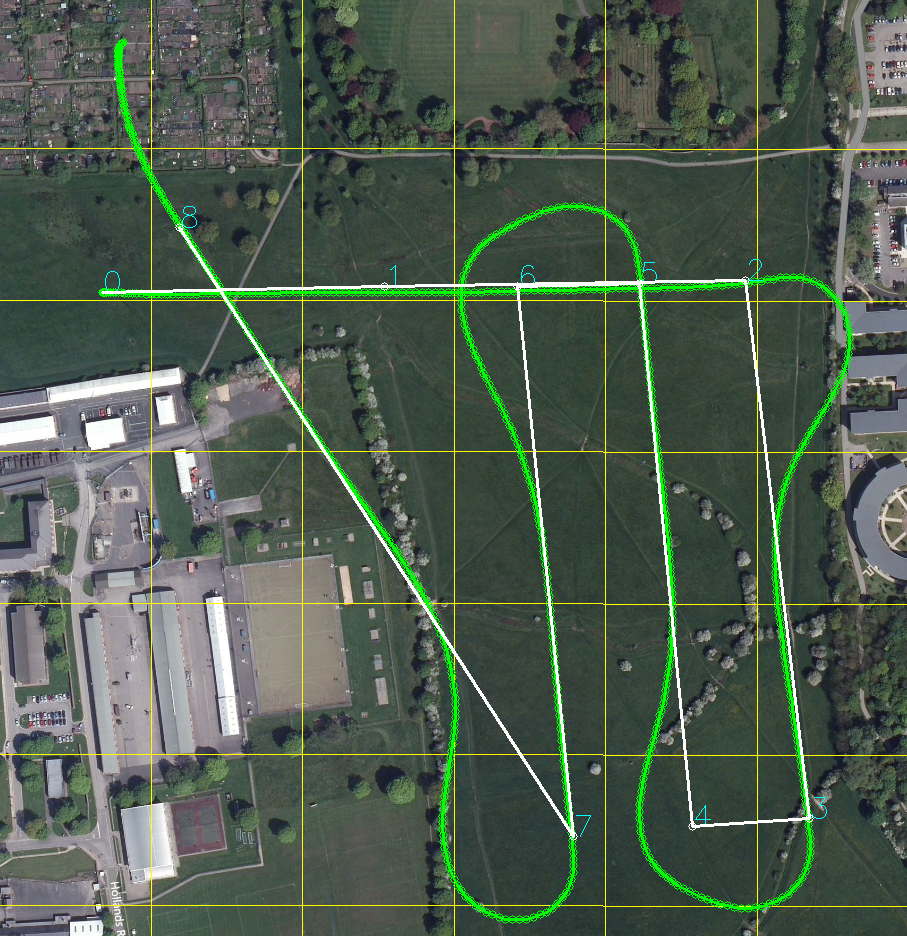
\includegraphics[width=0.8\textwidth]{BaseArduPlane}
\caption[Stock ArduPlane Path Tracking]{Results of a flight simulation using stock ArduPlane}
\label{fig:baseArduPlane}
\end{figure}

\begin{figure}[htbp!] 
\centering    
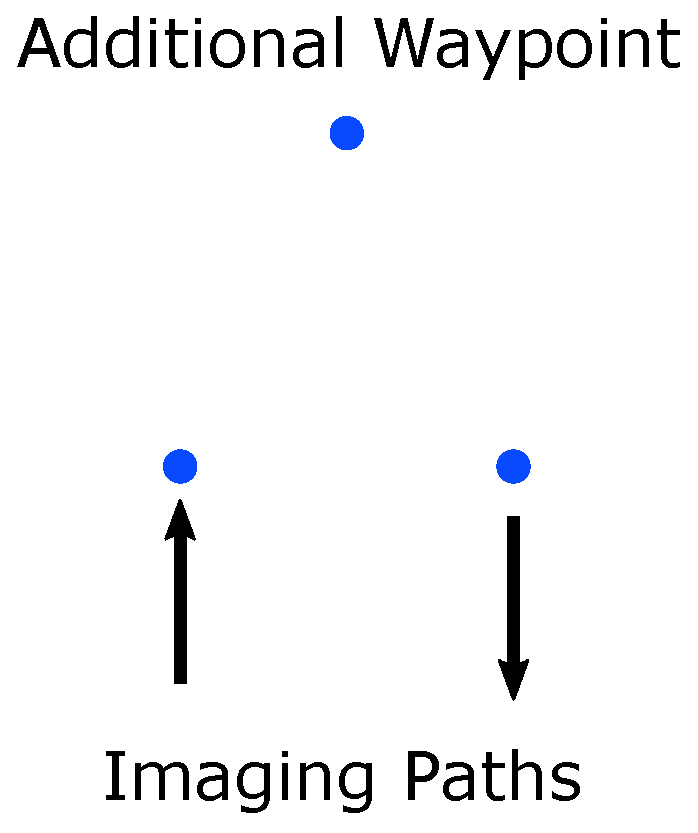
\includegraphics[width=0.4\textwidth]{WaypointManipulation}
\caption[Aligning With an Imaging Path in Stock ArduPlane]{One solution for aligning with an imaging path in the current version of ArduPlane via waypoint manipulation}
\label{fig:waypoingmanipulation}
\end{figure}

One of the problems we have is that ArduPlane navigates via straight lines drawn between points and has no concept of pre-emptive flight control or prioritisation of path sections. We can utilise Dubins paths as described in Section \ref{litrev:dubins} to decribe the shortest path possible between imaging paths that take the orientation of the UAV into consideration. We can then extend this work using the research discussed in Section \ref{litrev:path} to also handle the effects of wind on navigation. Using these techniques, we can introduce extra navigation steps at the planning stage that will in effect prioritise our imaging paths by ensuring the UAV arrives at the start of the path with the correction orientation and direction of travel. If a solution were to be implemented into the mission planning software, it would enable the user to specify the start and end points of imaging runs, and automatically calculate the desired Dubins path between them. 

As mentioned in Section \ref{intro}, this project is being run in parallel with another project investigating a related area of work. This other project is interested in path optimisation, for which one important feature is of course length. It was decided that this optimisation research should utilise the results of this work when calculating path lengths, suggesting the integration of the two projects at a later date. The result of this is that an additional aim for this task is to be able to share the system generated here for use in other work. It was decided that the best way to do this would be to create a standalone console application that could be compiled and shared, which took a number of parameters and returned details about the resulting paths. This shall be discussed further along with the other implementation work.

In effect we aim to introduce a new turning technique to the autopilot system, and the first stage of completing this is to be able to plan paths that define these turns. The result of this work will be effectively replacing the straight lines currently joining the ends of imaging paths with curved turns in the form of Dubins paths. We place no importance on the route travelled between the imaging paths, so we can replace the current paths with our own in order to prioritise aligning with imaging paths. By utilising Dubins paths we will also be improving battery life, as by their very definition DUbins paths are the shortest suitable routes we can take. 

We can summarise our aims for this task as covering the following points:

\begin{itemize}
	\item Being able to calculate suitable Dubins paths for a given UAV platform, taking into consideration its turning radius
	\item Being able to calculate suitable Dubins paths for a given UAV platform flying in a given wind condition
	\item Being able to define the resulting Dubins paths segments, either via location or length
	\item Allowing a user to specify a start and end point with prescribed orientation for our Dubins paths in all scenarios
	\item Creating a standalone application to share the results of this work
\end{itemize}


As we can infer from the aims above, this task needed to be completed in a number of steps. To achieve this, the overall path planning tasks was split up into a number of stages, the order in which these were carried out is as follows:

\begin{enumerate}
	\item Plot Dubins paths in MATLAB
	\item Plot the effect of a given wind input on the ground relative plot of the same Dubins paths
	\item Implement a system to select an air relative Dubins path that results in the ground relative path tracking to our desired location and orientation
	\item Implement this system as a standalone console application
\end{enumerate}


Throughout all stages of this task it was important to test the completed work to ensure we were prepared to move onto the next step. This was also important so as to minimise the risk of carrying bugs and errors forward throughout the project. 

%TODO finalise aims
%******************************************************************************************************
%******************************************************************************************************
\section{Path Planning - Stage 1: Plotting Dubins Paths in MATLAB}
\label{task1:stage1}

\subsection{Stage 1: Design}
\label{task1:stage1:design}


The design process for this task was very simple, as the author was aware of the availability of the C based Dubins path application and associated MATLAB wrapper \cite{WalkerDubinsCurves,MexDubinsCurves}. From the start the author was aware of the risk of using unverified work, however by analysing the source code and comparing the mathematical calculations with those found in \cite{shkel2001classification}, it was deemed suitable to progress using these resources. After this analysis of the supplied code, the only work left in order to complete this stage would be to supply inputs to the Dubins application, process outputs, and plot the results.

Throughout this stage we need to ensure that we are able to supply any combination of inputs to the program, specifying locations and orientations for both ends of the Dubins path as well as turning radius for our UAV.

\subsection{Stage 1:Implementation}
\label{task1:stage1:implementation}


This stage was, as expected, very straightforward. The first step was to first analyse the MATLAB Mex wrapper to ensure it was written as expected. Before using MATLAB's Mex function to convert the C\texttt{++} file into a MATLAB function, the \textit{dubins\_LSL}, \textit{dubins\_RSR}, \textit{dubins\_LSR}, \textit{dubins\_RSL}, \textit{dubins\_RLR}, and \textit{dubins\_LRL} functions were compared with \cite{shkel2001classification}. Thankfully the formulae and path length calculations matched up so were considered reliable. 

There was, however, one error found in this C\texttt{++} file. The main function which calls the calculation functions is called \textit{dubins\_init\_normalised}, and is responsible for both initialising, calculating, and assessing all of the path types. The problem was found in the following code snippet: 

\begin{minipage}{\linewidth}
\begin{lstlisting}[language=C++]
    int bestType = 0;
    double minCost = results[0][3];
    for(int i = 1; i < 6; i++) 
    {
        if( results[i][3] < minCost ) {
            minCost = results[i][3];
            bestType = i;
        } 
    }
\end{lstlisting}
\end{minipage}

This section of the \textit{dubins\_init\_normalised} function was responsible for looping through all of the path length values and selecting the shortest path which would then be returned from the program. In the \textit{for} loop, the \textit{i} variable was initialised with a value of 1, when it should have been initialised as 0. If this error had not been picked up, it would have meant that the program would never assess the result for the LSL path type, regardless of whether or not it was the shortest. This obviously would have been an issue, we most likely would have still been able to find Dubins paths to fit our requirements, but removing an entire path type could not have been beneficial. 

Once the Dubins Mex application was built, it was very simple to use. The inputs to the function are:
\begin{itemize}
	\item $q_0$ : x co-ordinate, y co-ordinate, orientation
	\item $q_1$ : x co-ordinate, y co-ordinate, orientation
	\item $radius$
	\item $stepSize$
\end{itemize}

where the orientation value is measured in radians increasing anti-clockwise from 0 pointing along the x-axis in the positive direction. The radius value is the minimum turning radius of our UAV, and the stepSize is effectively the resolution at which we want to take measurements. Throughout this project the $stepSize$ value has been set at 0.1, corresponding to a data point being calculated every 0.1 units along the Dubins path. The function returns an array with three rows; the x co-ordinates, the y co-ordinates, and the orientation of the UAV at each data point. By simply plotting the x and y co-ordinates, we have printed out the shortest Dubins path for the given input parameters. 

It is worth mentioning at this point that strictly speaking in this scenario, and for all the project work completed in MATLAB, the units are essentially arbitrary. It is easiest to assume however that everything is measured in metres, however we could be working with any measurement of distance. Thus we shall be treating both co-ordinates and radii as being measured in metres henceforth.

Fig. \ref{fig:pp1demo} shows the output of this program when given the following parameters:

\begin{itemize}
	\item $q_0 = 0, 0, \pi/2$
	\item $q_1 = 10, 10, 3\pi/2$
	\item $radius = 25$
	\item $stepSize = 0.1$
\end{itemize}


\begin{figure}[htbp!] 
\centering    
\includegraphics[width=\textwidth]{PP1_Demo}
\caption[stage 1: Plotting Dubins Paths in MATLAB]{The plot results of stage 1 in MATLAB demonstrating a simple RLR Dubins path}
\label{fig:pp1demo}
\end{figure}

\subsection{Stage 1: Testing}
\label{task1:stage1:testing}

The primary testing phase for this stage was in fact more of a quality assurance process, stepping through the Mex application ensuring that the path formulae matched that of the research it was based on. This did pick up a small error, proving that it was a worthwhile endeavour. 

Other than this, the testing process was limited to supplying a variety of inputs to the MATLAB code and visually inspecting the output plot. One slight problem that was found was that if the co-ordinates of the start and endpoints were identical, no path was calculated and plotted. To get around this we simply needed to ensure that the co-ordinates differed, if only by a miniscule amount. 


%******************************************************************************************************
%******************************************************************************************************
\section{Path Planning - Stage 2: Plotting the Effects of Wind on Dubins Paths}
\label{task1:stage1}

\subsection{Stage 2: Design}
\label{task1:stage2:design}

The next step for us to calculate the ground relative path followed by the UAV when commanded to fly a Dubins path in a wind condition. Regarding the air relative frame of reference, the UAV will be simply flying a Dubins path, however if we were to examine the GPS location data we would instead be seeing the UAV having flown a different path entirely. This stage is designed to be completed in MATLAB and to extend the capabilities of the program developed in stage 1. Alongside the original Dubins path plot we should plot the wind-affected path so as to easily allow comparison between the two. The plot should also display information about the wind vector to help visual inspection of the resulting paths. 

\subsection{Stage 2:Implementation}
\label{task1:stage2:implementation}

For this stage we needed to plot a Dubins path as before, but additionally plot its ground relative counterpart, calculated using a wind input. This required two additional parameters, the airspeed of the UAV, and a wind vector. 

The Dubins Mex application takes a value $stepSize$, used to calculate the distance along the path between every set of co-ordinate values. We also know that the application returns a $3 \times n$ array as its output. The $n$ value is very simply calculated in MATLAB, indicating how many location readings have been taken.

Using these values along with the input to define the airspeed of the UAV, we can calculate the time delta between each reading as follows:

\begin{equation}
	timeDelta = \frac{1}{(\frac{uavSpeed}{stepSize})}
\end{equation}

At this point we now know the time difference between each reading and are ready to start adding the effects of wind. To massively simplify the mathematics involved in calculating wind effects, it was decided that the best approach was to normalise all other parameters to allow the wind vector to always act along the x axis. This works because using our 3 parameters for each end of the path, we can still describe any possible configuration when limiting the wind to act in only one direction. As such, the wind vector is simply a positive or negative value, which is used to define the wind speed and direction. A negative value for the wind vector indicates wind blowing in the negative direction along the x axis, and vice versa for a positive value. Using this, we can enter the following very simple loop to calculate the effects of wind:

% \begin{frame}
\begin{center}
\begin{minipage}{\linewidth}
\begin{algorithm}[H]
\label{pp2Algorithm}
\SetAlgoLined
	timeCounter = 0\;
	\For{i from 1 to n}{
	path(4,i) = timeCounter\;
	path(5,i) = path(1,i) + (timeCounter * windVector)\;
	timeCounter = timeCounter + timeDelta\; 
	}
\caption{Calculating the the shape of a path subject to wind}
\end{algorithm}
\end{minipage}
\end{center}
% \end{frame}

This algorithm works by adding two additional rows to the output matrix from the Dubins Mex program, the first of which we populate with the time value corresponding to the data points in that column, and the second we populate with the new x values for the ground relative path. As mentioned, we do not need to calculate the y values for the ground relative path, as the wind is blowing in the x direction. Because of this we can simply calculate the offset in the x direction as a result of wind by multipling the time the UAV has been flying for with the wind vector, and adding this to the x location of the air relative path. Following this we simply plot both paths on the same graph, adding a legend and an arrow to show the wind vector, and we have Fig. \ref{fig:pp2demo}

\begin{figure}[htbp!] 
\centering    
\includegraphics[width=\textwidth]{PP2_Demo}
\caption[stage 2: Plotting the Effects of Wind on Dubins Paths in MATLAB]{The plot results of stage 2 in MATLAB, showing the ground relative path corresponding to an air relative Dubins path}
\label{fig:pp2demo}
\end{figure}

The inputs for the results seen in \ref{fig:pp2demo} are exactly the same as for the test carried out in Section \ref{task1:implementation:stage1}, with the addition of a wind vector value and a UAV airspeed value. The airspeed chosen for the UAV was 18 metres per second, as this was the cruising speed of the UAV used by Dr Andrew Pomfret on his expedition to Svalbard. A windspeed of 10 metres per second was used, blowing in the negative x direction.

\subsection{Stage 2: Testing}
\label{task1:stage2:testing}

As we had specified throughout that the wind vector was always pointing along the x axis, it was very easy to calculate expected offset in the x direction between the two paths as a result of wind. At the end of the MATLAB file for this stage we print out:

\begin{itemize}
	\item The start point of both paths and their orientation, equal to the values of $q_0$
	\item The location and orientation of the end point of the air relative path, equal to $q_1$
	\item The location and orientation of the end point of the ground relative path
	\item The duration of the flight in seconds
	\item The expected offset in the x axis as a result of wind. This was calculated by multiplying the wind vector with the flight duration
	\item The actual offset in the x axis, calculated as the distance between the end points of the two path types
\end{itemize}

By printing out this information and running a number of tests, it was easy to quickly check that we were infact calculating a correct offset due to wind, all within the MATLAB console. 

%******************************************************************************************************
%******************************************************************************************************
\section{Path Planning - Stage 3: }
\label{task1:stage3}

\subsection{Stage 3: Design}
\label{task1:stage3:design}


This stage is where we finalise our new path planning system. For the application of aerial photography, the frame of reference that is most relevant to us is the ground relative frame. We want to be able to command the UAV to a location above a certain point on the ground, not a certain point in air. As such, we to implement a system that takes a desired destination, and calculates the air relative Dubins path. This Dubins path must of course take wind into consideration, as well as UAV orientations at either end of the turn alongside the UAV turning radius. Once again this is to be implemented entirely in MATLAB. 

This will use a similar plot style to that produced in stage 2, allowing us to compare air and ground relative paths as well as the wind vector. This will hopefully enable us to quickly spot any glaring errors, as well as do some rudimentary estimations on whether the effect of wind is being calculated correctly.

This system will be heavily based on the research discussed in Section \ref{litrev:path}, implementing the search algorithm as mentioned.

\subsection{Stage 3:Implementation}
\label{task1:stage3:implementation}

For this iteration of our path planning system, we need to implement our search algorithm to find a suitable air relative path to lead our UAV to the correct groud relative position. In this section we introduce the use of a virtual target, $vt$. The input parameters for this system are the same as in stage 2. 

In stage 2, we simply defined a Dubins path between $q_0$ and $q_1$ and then calculated the effect of wind on the resultant path. In this solution, we define an air relative dubins path between $q_0$ and $vt$, that when coupled with the effect of wind, will produce a ground relative path between $q_0$ and $d$. This will allow us to specify the end point of our first imaging path, $q_0$, and the start point of the next imaging path, $d$. 

This search algorithm works using a series of time values which we compare to assess the suitability of a proposed solution. The algorithm starts at time 0, and at this point the UAV is at $q_0$ ready to begin its path, and $vt$ is equal to $d$. $vt$ is an air relative position, so as soon as the timer starts counting, its position changes following a vector equal and opposite to the wind vector. 

Our search algorithm solution is claculated based off two time measurements, $Ta$ and $Tvt$. $Ta$ is the time taken for the UAV to travel from $q_0$ to $vt$ by flying a Dubins path, so can be calculated using:

\begin{equation}
	Ta = \frac{(n*stepSize)}{uavSpeed}
\end{equation}

Where $n$ is the size of the  $3 \times n$ array returned by the Dubins Mex application, and $stepSize$ is the resolution value we are using.

$Tvt$ is the time taken for the virtual target to move from its start position to its current position, so is simply calculated as the time that the algorithm has been running. The following code listing is an excerpt from the finalised solution:

\begin{minipage}{\linewidth}
\begin{lstlisting}[language=MATLAB]
% Ta starts as the time taken for the UAV to travel from q0 to d as if there was no wind, so
noWindPath = dubins(q0,d,radius,stepSize);

% Calculate Ta using the stepsize (distance between each datapoint generated by dubins function), and speed of uav.
% Number of x position readings * stepsize = length of path
Ta =  (numel(noWindPath(1,:))*stepSize)/uavSpeed; 

% Calculation time is 0 when turn starts
% At time 0 UAV is at q0
% At time 0 vt = d, therefore Tvt = 0  too;
calculationTime = 0;
Tvt = calculationTime;

%% Search algorithm
while ((Ta-Tvt)>0.1)||((Ta-Tvt)<(-0.1))
    % Firstly increment our calculation time
    calculationTime = calculationTime + 0.1;
    % Then update the location of the vt. vt(1) is the x co-ordinate value, this works because wind is always in only the x direction
    % Note: *0.1 because we are evaluating this 10 times for every second of calculationTime
    vt(1) = vt(1) + 0.1*vtVector;
    % Tvt is the time it has taken for the vt to move from d to its current location, so is equal to calculationTime
    Tvt = calculationTime;
    % Create a candidate dubins path, to see if this position of vt is a suitable solution for the search
    candidatePath = dubins(q0,vt,radius,stepSize);
    % Recalculate Ta using the new candidatePath
    Ta = (numel(candidatePath(1,:))*stepSize)/uavSpeed;
end
\end{lstlisting}
\end{minipage}

Once the for loop exits we consider the algorithm solved and call another function to plot the results. The function we call is essentially a clone of the function created for stage 2, modified to take additional parameters. We pass in:

\begin{itemize}
	\item $q_0$ location and orientation
	\item $vt$ location and orientation
	\item $radius$
	\item $windVector$
	\item $uavSpeed$
\end{itemize}

The result of this can be seen in Fig. \ref{fig:pp3demo}, where the inputs were exactly the same as for stage 2, however instead of $q_0$ having the values $(10,10,3\pi/2)$, we specify $d$ as having these values.

\begin{figure}[htbp!] 
\centering    
\includegraphics[width=\textwidth]{PP3_Demo}
\caption[stage 3: Generating an Air Relative Path Based on Desired Ground Relative Destination in MATLAB]{The plot results of stage 3 in MATLAB, showing the air relative path calculated from a desired ground relative end point}
\label{fig:pp3demo}
\end{figure}


\subsection{Stage 3: Testing}
\label{task1:stage3:testing}

By printing out the same information as printed out before, we can very easily see two important things; as before that we are calculating the correct wind offset, and that the ground relative path ends at the desired $d$ location. We can also compare the location of the $vt$ with the end point of the air relative path to ensure that we are still creating a correct Dubins path. All of this combined ensures that we can be confident that our algorithm is working, and that we are able to find an air relative path from a desired endpoint of the corresponding ground relative path. 

Other than this, as before, a number of scenarios were tested and visually inspected to ensure the path shapes were as expected.

%******************************************************************************************************
%******************************************************************************************************
\section{Path Planning - Stage 4: }
\label{task1:stage4}

\subsection{Stage 4: Design}
\label{task1:stage4:design}

The final step for completing the path planning part of this project is to create the console application. This console application will serve three main purposes; firstly it will form an integral part of path length calculation in the other project relating to this work, mentioned in Section \ref{intro}. Secondly it will enable us to do some fast and thorough testing of our path generation search algorithm, as will be discussed later. Finally, it will be used in the testing stages of the second task in this project, the path following task.

\subsection{Stage 4:Implementation}
\label{task1:stage4:implementation}

The last work to complete for this task was to create a standalone console application version of the code in stage 3. This did not need to generate any plots, but must return the lengths of each segment of the chosen Dubins path. 

To simplify the development process, instead of converting the code from the Dubins Mex application, we used the original source code available at \cite{WalkerDubinsCurves}. Because the purpose of a Mex wrapper is to provide compatability with MATLAB, the input and output handling is designed to work using MATLAB data structures and functionality. The original source code is a pure C application, which was more straightforward to convert to a console application. The resulting application was written in C\texttt{++} so as to simplify the handling of strings, as we needed to be able to display to the user the path type (e.g. LSL, RSL), and using C would make this more complicated. 

The research documented in \cite{mcgee2005optimal} draws two major conclusions;

\begin{enumerate}
	\item For the majority of cases, one of the 6 types of regular Dubins path will satisfy the equation $Tvt = Ta$
	\item For the remaining cases, the path that must be flown will be a non-optimal path, meaning the path must be lengthened 
\end{enumerate}

Due to conclusion one, \textit{dubins.cpp} was modified from the source code available on GitHub to instead return an array of Dubins paths, populated with all 6 path types. This would ensure that we could check to see if any of the paths for the chosen $vt$ position satisfied our equation. The initial intention was to stay true to the referenced research, attempting to find paths that satisfied $Tvt = Ta$. In the first version of this application, we did not supply any method for handling scenarios described by conclusion two in purpose. The intention was to perform a series of tests to determine how frequently we would need to fly non-optimal paths, and adjust our path calculations accordingly. This testing will be discussed in \ref{task1:testing:stage4}. The findings, however, suggested that by allowing a difference of up to 0.1 seconds, that we could solve the algorithm for all scenarios tested using the regular Dubins paths. 

This 0.1 second tolerance introduces an error into system, resulting in the UAV not quite aligning with $d$ in certain situations. However, if using a relatively fast UAV that has an airspeed of 30 metres per second flying a path that has the maximum error value, you will only miss the mark by 3 metres. When we consider that most aerial photography will be conducted at more than 20 metres above ground, this level of error is not very large. By allowing this small margin of error, we simplified both the path planning and path following sections of this project, so it was considered worth sacrificing a little performance for simplicity and processing speed.

%TODO go back and explain how this was included into PP2/PP3

The original Dubins path code can be found in \textit{dubins.cpp} which has been modified by the author to fit our purposes. There were a number of functions that were copied and altered to return all 6 path types, using the \textit{DubinsPath} structure found in \textit{dubins.h}. 

The finalised search algorithm is very similar to that developed in stage 3, converted to operate using C\texttt{++} syntax and program flow. In this implementation however, we then proceed to print out information regarding the solved path, as can be seen in Fig. \ref{fig:consoledemo}.

\begin{figure}%[htbp!] 
\centering    
\includegraphics[width=\textwidth]{Console_Demo}
\caption[Screenshot of the finalised console application]{A screenshot of the console application, as seen by the user}
\label{fig:consoledemo}
\end{figure}

At a later stage in this project, another version of this console application was developed to take the orientation inputs in degrees rather than radians, and to display flight times for each segment as milliseconds rather than seconds. This was done mainly for the authors convenience, and was used to speed up the testing cycle of the path following section of this work. A screenshot of this modified console can be seen in Appendix %TODO appendix degrees console

\subsection{Stage 4: Testing}
\label{task1:stage4:testing}

The testing for this stage was far more extensive than the previous stages, and for good reason, as it would be the tool used for all testing in the next task in the project. As discussed before, the results of the first stage of this testing altered the search algorithm at the centre of all of this work, resulting in quicker and simpler development. The way this was done was to create another application, using exactly the same search algorithm, and test a very broad range of scenarios. This second application, called \textit{AlignTest}, called the search algorithm thousands of times, each time with unique inputs, and printed the results to a file. These inputs were made up of all possible combinations of:

\begin{itemize}
	\item Wind vector integer values from -9 to 9 inclusively
	\item $d$ location x co-ordinates of 0, 15, 30, 45, 60, 75, and 90
	\item $d$ location y co-ordinates of 0, 15, 30, 45, 60, 75, and 90
	\item $q_0$ location orientations of integers between 0 and 7 inclusively
	\item $d$ location orientations of integers between 0 and 7 inclusively
\end{itemize}

The constant values were:
\begin{itemize}
 	\item $q_0$ starting at the co-ordinates 0,0
 	\item Turn radius of 25 metres
 	\item UAV airspeed of 18 metres per second
 	\item Step size of 0.1 (as always)
 \end{itemize} 

 The UAV speed parameters and turning radius were once again chosen to emulate the UAV used by Dr Andrew Pomfret on his Svalbard expedition.

These scenarios were all tested using the following nested loops:

\begin{minipage}{\linewidth}
\begin{lstlisting}[language=C++]
for (int dx = 0; dx < 91; dx += 15) {
    for (int dy = 0; dy < 91; dy += 15) {
        for (int wspd = -9; wspd < 10; wspd++) {
            for (int dOrient = 0; dOrient < 8; dOrient++) {
                for (int qOrient = 0; qOrient < 8; qOrient++) {
                    d[0] = dx;
                    d[1] = dy;
                    d[2] = dOrient;
                    q0[2] = qOrient;
                    calculatePaths (r, q0, d, stepsize, speed, wspd);
                }
            }
        }
    }
}
\end{lstlisting}
\end{minipage}

The results of each testing scenario were printed to a text file for simple processing after. This is an example of one entry:

\begin{minipage}{\linewidth}
\begin{lstlisting}[language={}]
Start: 		0, 0, 7
End: 		60, 30, 5
Wspd: 		-3
Vt:  		77.4, 30, 5
Path type: 	LSR
Section 1: 	3.4326
Section 2: 	48.9462
Section 3: 	53.4326
Total: 		10.2978
\end{lstlisting}
\end{minipage}

Where ``Start'' is the $q_0$ location, ``End'' is the $d$ location, and ``Wspd'' is the windspeed vector value, with its sign denoting direction in the x axis. The path type is printed out and then the $t$, $p$, and $q$ segment lengths are printed too. 

This set of tests covers 59584 unique testing scenarios including 3136 no-wind scenarios, 28224 positive wind vectors, and 28224 negative wind vectors. As can be seen in the source file \textit{calculatePaths.cpp}, the search algorithm has a built-in timeout feature, where if the turn would take longer than 30 seconds to complete, we print an error to the text file suggesting no suitable path has been found. By introducing the 0.1 second error allowance in the comparison between $Tvt$ and $Ta$ we were able to test all 59584 scenarios without a single instance of a suitable path not being found. This finding allowed us to go back to stage 3 of this work and introduce this allowance here too, so as to ensure continuity throughout the work. 

The final stage of testing for this task was to compare results produced by our MATLAB solution with those of the console application. By manually entering the same input parameters into both, we were able to run a series of checks to guarantee this. The first check is to ensure that the plotted path is of the same type described in the console window (e.g. LRL). Following this, we also edited the MATLAB file to print out the length of path, which we could then compare to the total provided by the console application. Allowing for very small margins of error due to rounding differences between MATLAB and C\texttt{++}, all scenarios checked presented the same results. With all of this complete, we were confident in our findings, and ready to progress to the next task in the project.

%******************************************************************************************************
%******************************************************************************************************
\section{Path Planning - Summary and Conclusions}
\label{task1:summary}
%TODO duhhh